\paragraph{Example 1}{
\begin{lstlisting}[language=Python]
from BNumMet.NonLinear import zBrentDekker
fun = lambda x: x**2 - 2
interval = [1, 2]
sol, nIter = zBrentDekker(fun, interval, iters = True)
print("Brent-Dekker method: x = %f, nIter = %d" % (sol, nIter))

>> Brent-Dekker method: x = 1.414214, nIter = 7
\end{lstlisting}
}
\paragraph{Example 2}{
\begin{lstlisting}[language=Python]
f = lambda x: sp.jv(0, x) # Bessel function of the first kind of order 0
interval = lambda n: [n * np.pi, (n + 1) * np.pi] # Interval for the n-th zero

zeros = [ zBrentDekker(f, interval(n)) for n in range(0, 10)]


x = np.arange(1, 10 * np.pi, np.pi / 50)
y = f(x)
plt.plot(x, y)
plt.plot(zeros, np.zeros(len(zeros)), "ro")
plt.axhline(0, color="k")
plt.show()
\end{lstlisting}
\begin{figure}[H]
    \centering
    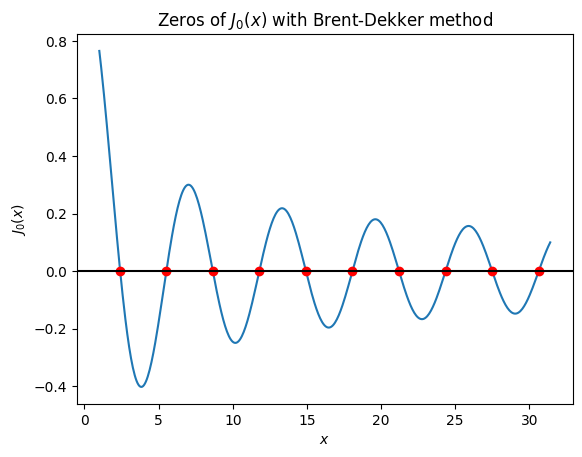
\includegraphics{Include/Images/Thesis/Documentation/NonLinear/Brentt-Dekker Example 2.png}
    \caption{Brentt-Dekker Example 2}
    \label{fig:Brentt-Dekker Example 2}
\end{figure}
}